% Use only LaTeX2e, calling the article.cls class and 12-point type.

\documentclass[12pt]{article}

% Users of the {thebibliography} environment or BibTeX should use the
% scicite.sty package, downloadable from *Science* at
% www.sciencemag.org/about/authors/prep/TeX_help/ .
% This package should properly format in-text
% reference calls and reference-list numbers.
\usepackage{hyperref}
\usepackage{scicite}
\usepackage{graphicx}
\usepackage{amsmath}
\usepackage{amsfonts}
\usepackage{setspace}
\usepackage{enumitem}
% Use times if you have the font installed; otherwise, comment out the
% following line.

\usepackage{times}

% The preamble here sets up a lot of new/revised commands and
% environments.  It's annoying, but please do *not* try to strip these
% out into a separate .sty file (which could lead to the loss of some
% information when we convert the file to other formats).  Instead, keep
% them in the preamble of your main LaTeX source file.


% The following parameters seem to provide a reasonable page setup.

\topmargin 0.0cm
\oddsidemargin 0.2cm
\textwidth 16cm 
\textheight 21cm
\footskip 1.0cm


%The next command sets up an environment for the abstract to your paper.

\newenvironment{sciabstract}{%
\begin{quote} \bf}
{\end{quote}}


% If your reference list includes text notes as well as references,
% include the following line; otherwise, comment it out.

\renewcommand\refname{References}

% The following lines set up an environment for the last note in the
% reference list, which commonly includes acknowledgments of funding,
% help, etc.  It's intended for users of BibTeX or the {thebibliography}
% environment.  Users who are hand-coding their references at the end
% using a list environment such as {enumerate} can simply add another
% item at the end, and it will be numbered automatically.

\newcounter{lastnote}
\newenvironment{scilastnote}{%
\setcounter{lastnote}{\value{enumiv}}%
\addtocounter{lastnote}{+1}%
\begin{list}%
{\arabic{lastnote}.}
{\setlength{\leftmargin}{.22in}}
{\setlength{\labelsep}{.5em}}}
{\end{list}}


% Include your paper's title here




% Place the author information here.  Please hand-code the contact
% information and notecalls; do *not* use \footnote commands.  Let the
% author contact information appear immediately below the author names
% as shown.  We would also prefer that you don't change the type-size
% settings shown here.




% Include the date command, but leave its argument blank.

\date{}



%%%%%%%%%%%%%%%%% END OF PREAMBLE %%%%%%%%%%%%%%%%



\begin{document} 

% Double-space the manuscript.

\baselineskip24pt
\setstretch{1.5}


% Make the title.









% In setting up this template for *Science* papers, we've used both
% the \section* command and the \paragraph* command for topical
% divisions.  Which you use will of course depend on the type of paper
% you're writing.  Review Articles tend to have displayed headings, for
% which \section* is more appropriate; Research Articles, when they have
% formal topical divisions at all, tend to signal them with bold text
% that runs into the paragraph, for which \paragraph* is the right
% choice.  Either way, use the asterisk (*) modifier, as shown, to
% suppress numbering.

\section{Introduction}

Wikipedia is an online project for the development of a freely accessible encyclopaedia \cite{O'Sullivan}. It is one of the most attractive platforms on the internet regarding the number of visitors and is ranked 5th  by the alexa.com, which is traffic ranking system worldwide\cite{alexa}. It has about 5.3 Million articles on English version and receives over 1.25 million edits daily. German wikipedia is the second-oldest with 2.1 Million articles and at present the second largest edition of wikipedia by number of articles. It has the second largest number of edits to exceed 100 million page edits\cite{german}. But then allowing anonymous edits is not so easy to maintain, nearly $7 \%$ \cite{potthast} of edits are vandalism, i.e. revisions to articles that decrease the quality and veracity of the content.\par Wikipedia is susceptible to vandalism by defining vandalism as 'editing (or  any other behaviour) deliberately intended to obstruct or defeat the project's purpose, which is to create a free encyclopaedia in a variety of languages presenting the sum of all human knowledge\cite{vandalism}.' Wikipedia is a dynamic resource that is constantly changed by its millions of editors. High visibility of its content is the main reason for vandalism. As anyone can edit wikipedia, there is no restriction to edit. Most of the time that's a good thing as millions of people have given positive contributions. But then there are also the problems like  children who can delete all its content and also some people who add incorrect information, deliberately or by mistake.



\section{User Access Levels}
As wikipedia grows continuously, it is increasingly infeasible for wikipedia users and administrators to manually protect articles. This is why several user groups are made and necessary rights are assigned to them to protect wikipedia articles. The user access level of an editor affects their ability to perform actions on wikipedia, depending on which user group rights are assigned to their account\cite{user}.
\subsection*{Unregistered User:}
These is the group of user who don’t have an user account in wikipedia. They are identified by IP address rather than username if any edits are made. These editors possess right to read and edit all pages in wikipedia except special pages and protected pages. They can upload files or images and also can create talk pages in any talk namespace.
\subsection*{Registered User :}
After creation of  user account, automatically user becomes registered user of wikipedia. These users can email other users after activation of email address. The editors from this user group can purge pages without a confirmation step. They can also save books to their user space.
\subsection*{Confirmed User:}
User accounts that are more than four days old and have made at least 10 edits are considered confirmed. These users can create articles, move pages, upload files, edit semi protected pages and upload a new version of an existing file.
\subsection*{Administrators : }
Administrators are volunteer editors who are granted the rights by the community by Request for Adminship (RfA) electing process. RFA process involves considerable discussion and examination of the candidate's activities as an editor. Administrators can perform page deletion, page protection, blocking and unblocking users and access to can modify fully protected pages.
\subsection*{Bureaucrats :}
Bureaucrat rights are granted by the community by Requests for Bureaucratship (RfB) electing process. Bureaucrats have technical and organisational duties like managing user databases etc. They have right to add or remove administrators and have extended rights of adding users to the bureaucrat user group. They can also flag and unplug bot account.
\subsection*{Rollback : }
Users of this user group can revert consecutive revisions of an editor using the 'rollback' feature. This right is automatically assigned to administrators.
\subsection*{Oversight and CheckUsers :}
They have right to delete and block screens through which they can hide revisions of pages from all other users. By using their special rights they can view a log of actions and the content of the hidden revisions. CheckUsers can view a list of all IP addresses used by a user account to edit the English wikipedia. A list of all edits made by an IP or all user accounts that have used an IP address. If passed through RfA or RfA-identical process, checkUsers can also have access to deleted revisions.
\subsection*{Bots:}
 Bot accounts are automated or semi-automated. The nature of their edits is well defined and they will be quickly blocked if their actions vary from  given tasks.
 \subsection*{Stewards :}
Stewards are appointed globally across all wikipedia. Users who are members of the steward user group may grant and revoke permission to or from any user in any other user group. Stewards can act as check-users, over-sighters, bureaucrats or administrators user to perform necessary action when required.
\section{Types of Vandalism  }
The main cause of Vandalism is purely based on the four primary actions. That is change in text, insert irrelevant text, delete text, and revert text in an article as in Fig.\ref{vandalismtypes}. Actions of delete, insert, and change involve the content and the formatting of articles as shown in Fig.\ref{Taxanomy}. The content class includes text, images and links whereas formatting includes HTML tags or CSS, and wikipedia templates.
Priedhorsky etal\cite{creating} categorised wikipedia damaged edits into seven types: Misinformation, Mass
delete, Partial delete, Offensive, Spam, Nonsense, and Other.
\begin{figure}[h]
\centering
\includegraphics[scale=0.45]{taxnomy.png}
\caption{Wikipedia action Taxonomy \cite{active}}
\label{Taxanomy}
\end{figure}
\begin{figure}[h]
\centering
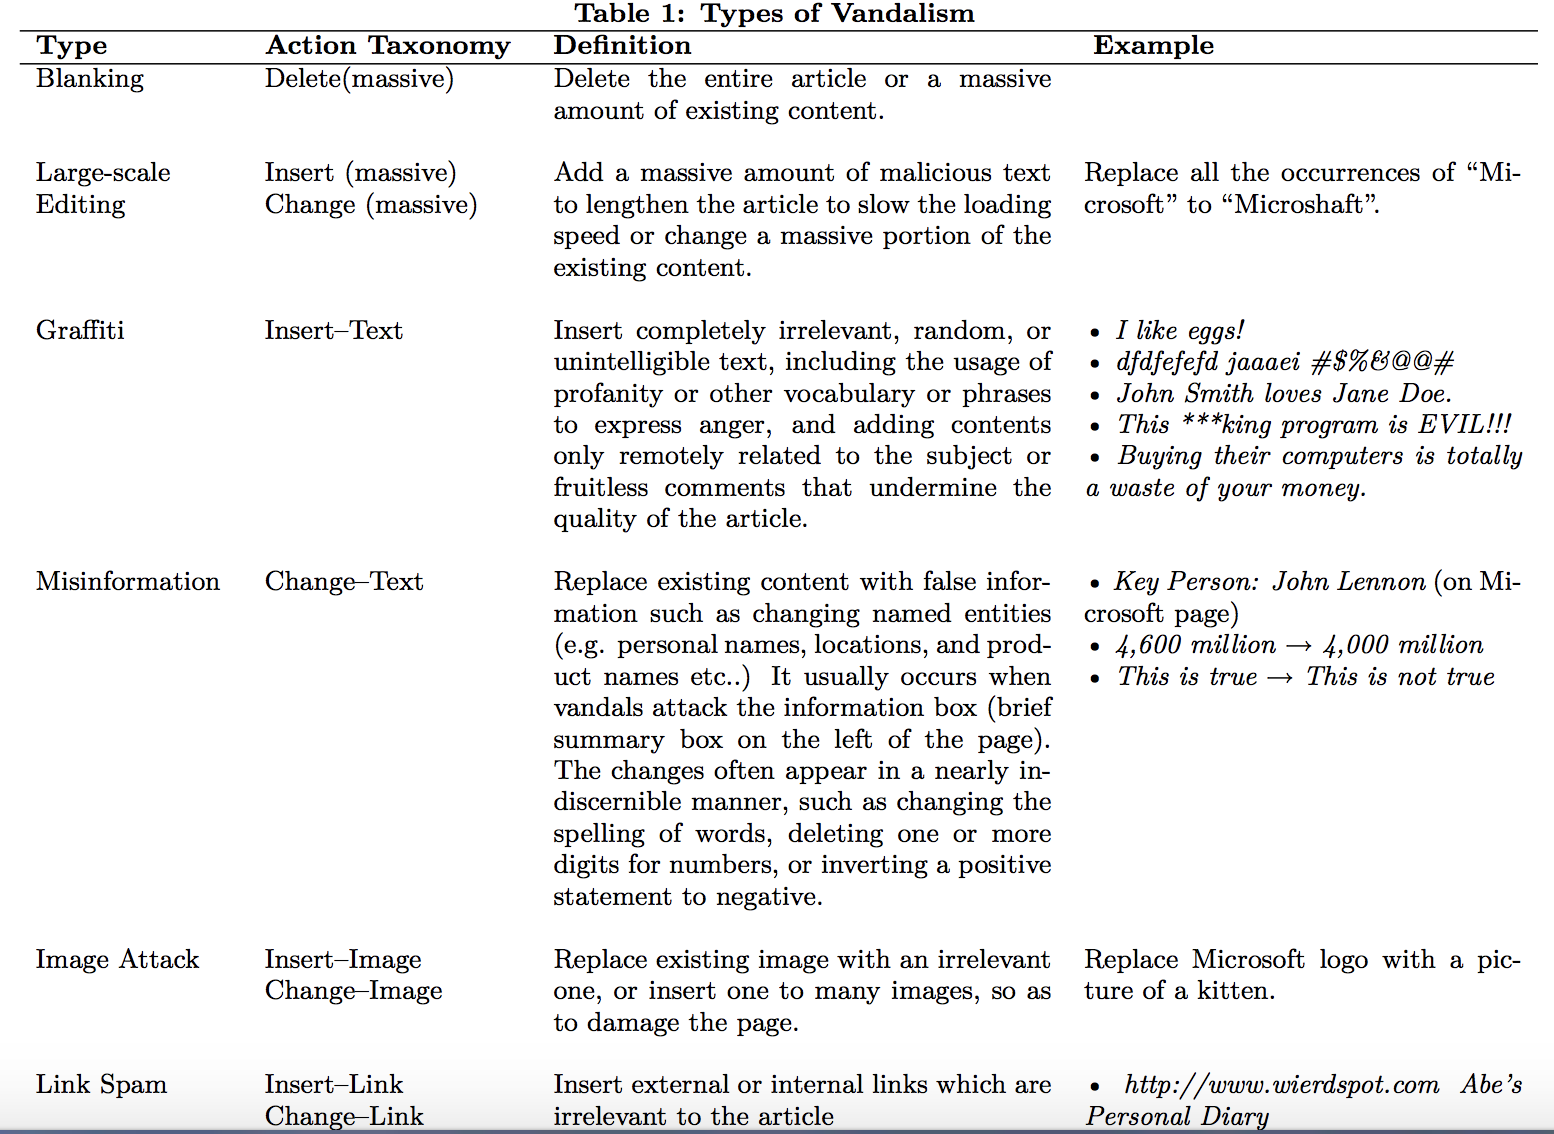
\includegraphics[scale=0.37]{vandalismtypes.png}
\caption{Types of Vandalism \cite{active}}
\label{vandalismtypes}
\end{figure}\\
Even though more rules can be generated to detect a list of commonly used vandalism language vocabulary (e.g. profanity, slang, unintelligible words etc.) but still it is difficult to maintain the list, as the vandalism language may change over time.Therefore, a rule-based filtering system to detect this type of vandalism is neither extensible nor easy to maintain.
\section{Notable acts of Vandalism}
There are many acts of wikipedia vandalism everyday on internet but here I am mentioning some interesting notable acts.
\begin{itemize}
\item[$\bullet$ ]In July 2015, when there were US elections. Many people were interested in this elections not only in USA but people all around the world. And then one person expressed his/her opinion by replacing entire Wikipedia page of Trump just by one sentence saying :'Let’s be fair, nobody cares about him' and vandalised it\cite{vandalism}.
\end{itemize}

\begin{itemize}
\item[$\bullet$ ]
\begin{figure}[h]
\centering
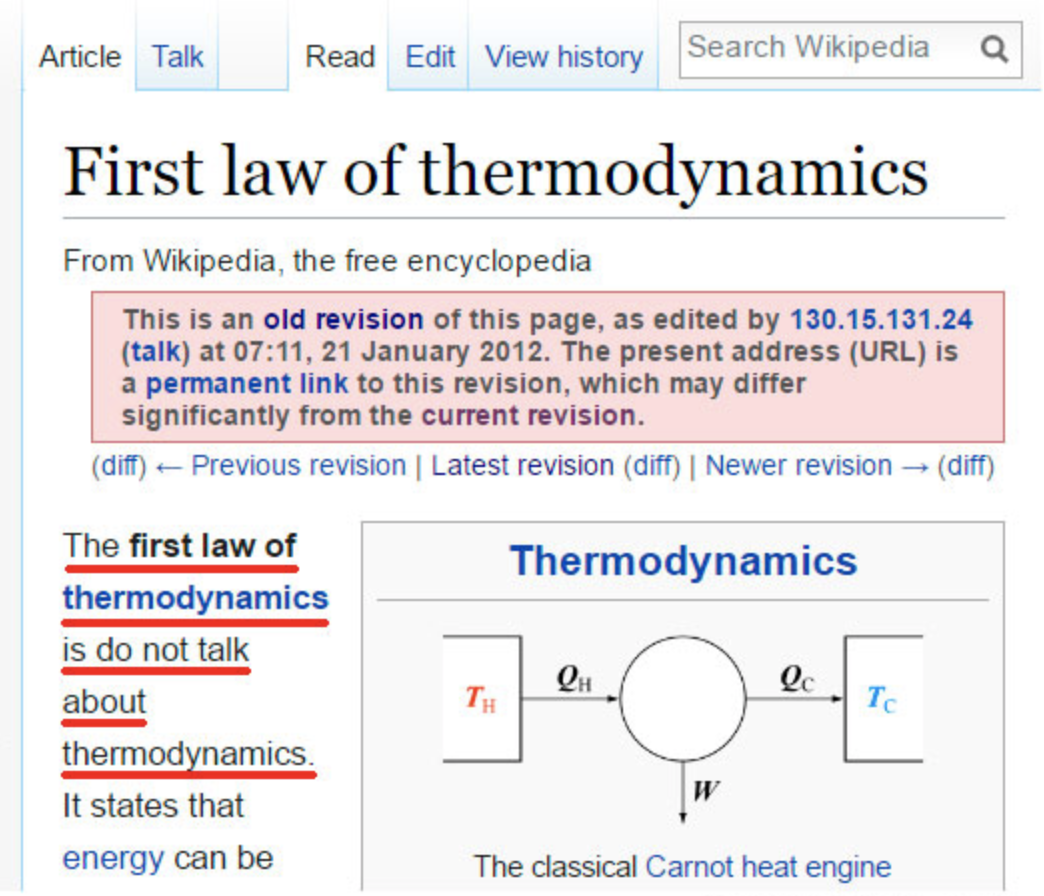
\includegraphics[scale=0.5]{thermodynamics}
\caption{Act of Vandalism \cite{vandalism}}
\label{thermodynamics.png}
\end{figure}
This Fig.\ref{thermodynamics.png} here shows how this wikipedia page is vandalised by adding  inappropriate text in between of an article. The content is inappropriate because all the users do not have same opinion towards the article. Wikipedia has a policy called “NPOV(neutral point of view)” which says that all the information on an article should be unbiased i.e no personal opinion should be expressed in an article.
\end{itemize}
\section{Vandalism detection methods}
Wikipedia keeps a record of everything\cite{help}. Below are the main benefits to have a record.
\subsection*{Responsibilty:}
Page histories help identify problematic edits and  editors who created those edits. Thousands of editors are warned every day for inappropriate behaviour of editing. Hundreds of user accounts are blocked every day for creating vandalism through adding incorrect information in text.
\subsection*{Reverting :}page history option is easy to use revert function (that is to reverse) another editor's inappropriate edit or even your own edit(if we made a mistake). Revert network of any article looks like the Fig.\ref{Revert} below. Here, nodes are editors and edges represent revert function used between the editors to change current version of an article at given time.
\begin{figure}[h]
\centering
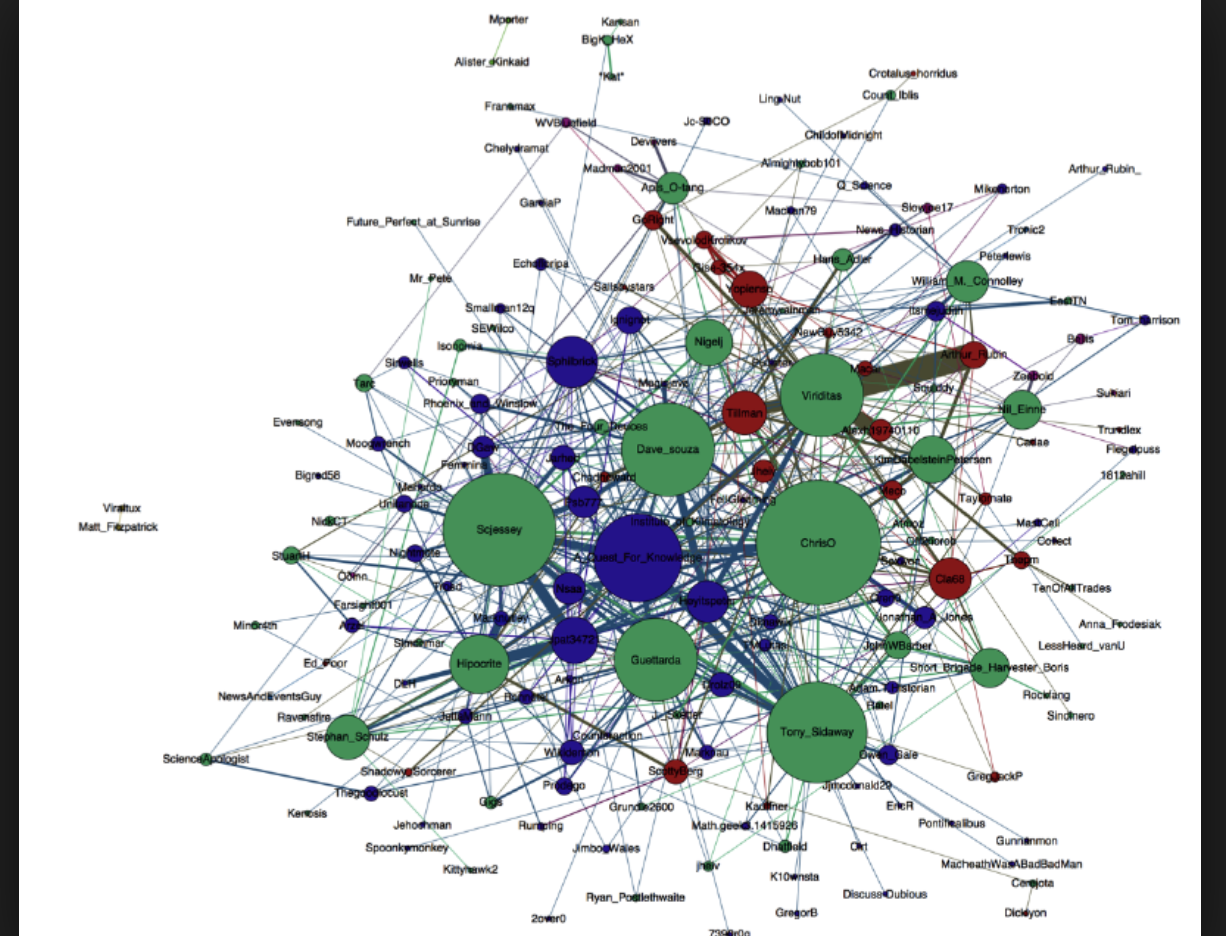
\includegraphics[scale=0.32]{Revert.png}
\caption{Revert network \cite{revert}}
\label{Revert}
\end{figure}
\subsection*{Reputation:}As edits will be visible to everyone and forever. Hopefully, editors will think twice before damaging the good work of others and because of that most of the editor's behave in good way as well.\\
Vandalism can be detected in both ways i.e manually and also by using automated bots.\cite{help} Bots uses regular expression and various rules to detect  the edit made was malicious or not. The database of wikipedia has a copy of every version of every page whether created or edited. By clicking on a page history tab, we can see the text on that page of every date and time. Each article in Wikipedia can be easily edited by using hyperlinks next to the text  and the changes made are visible immediately. A version history is available for each article along with the real name, user name or Internet address of the editor so that changes can be tracked and reverted easily. \\Registered authors can also keep a watchlist on pages to monitor changes to certain articles usually those to which they made a contribution themselves. Similarly there is a special page which lists all recent changes to any wikipedia article. These software features are designed to foster a system of continuous peer-review among contributors and even occasional readers of Wikipedia articles. Research suggests that this system may in fact help to improve the quality of articles and prevent obvious vandalism\cite{help}.
In the last decade, the free encyclopaedia Wikipedia has become one of the most valuable and comprehensive knowledge sources in Natural Language Processing\cite{anthology}. It has been used for numerous NLP tasks, e.g. word sense disambiguation, semantic relatedness measures, or text categorisation. Some researchers explore motivated approaches like applying Machine Learning and Natural Language Processing techniques to the task of vandalism detection\cite{Harpalani}. Much of previous work relies on hand picked rules such as lexical cues (ex: vulgar words) and metadata (ex: anonymity, edit frequency) to automatically detect vandalism in Wikipedia \cite{potthast}. To differentiate between the styles of normal users and vandalisers many researchers employ language models to capture the stylistic differences between authentic and vandalising revisions. Training of two trigram language model with Good-Turing discounting and Katz backoff for smoothing of vandalising edits  which is based on the text difference between the vandalising and previous revision and good edits based on the text difference between the new and previous revision in an article\cite{Harpalani}.The system also decides if an edit to an article is vandalism by training a classifier based on a set of features i.e based on metadata or sentiment derived from many different aspects of the edit.
\section{Conflicts among wikipedia Users}
Conflict in wikipedia is very common among editors as their opinion collide a lot. Research has measured wikipedia conflict at two levels: 
\begin{itemize}
\item[$\bullet$ ]Single articles and
 \item[$\bullet$ ]Categories of pages.
\end{itemize}
Some conflicts are observed within small groups of articles identifying their frequency, size and intensity. Also individual conflicts spanning multiple articles and effects of conflict upon user's editing habits\cite{char}.While most conflicts are of low intensity which takes place in a single article, high-intensity conflicts frequently span multiple articles. However, conflict can also be disappointing by discouraging volunteers and leading them to stop contributing.
Mainly there are four major conflicts among users of Wikipedia \cite{main} as mentioned below:
\subsection*{Edit War:} Edit wars are a common phenomenon in the area of political conflict in wikipedia especially in disputed areas like politics, religion, or other morally loaded issues which are very prone to conflict. Editors who are attention seekers or stubborn editors willing to their own point of views. Ex: If there are group of people together who are talking about religion or about their countries  then  obviously conflict arise between them. Likewise there are lot of editorial wars among editors. But,the good thing about wikipedia is that all this records in revision history i.e the interaction between editors and how the articles are changing over time and is visible. Most of the time revert function is actually used to fight and to pursue their own opinions against other editors.                                                                           Edit wars are usually handled by administrators either by blocking an article or a discussion page from being edited or by temporarily revoking the right to edit wikipedia for one or both edit warriors. Repeated edit wars can also result in the definite exclusion of edit warriors from the project.
\subsection*{Simple Vandalism:} Simple vandalism occurs majorly from new users, who are eager to try new things out and mostly it include cases of blatant vandalism. But in this type of conflict, the scope of disagreement is much less compared to other conflict types which are very much prone for disputes.\\
\begin{figure}[h]
\centering
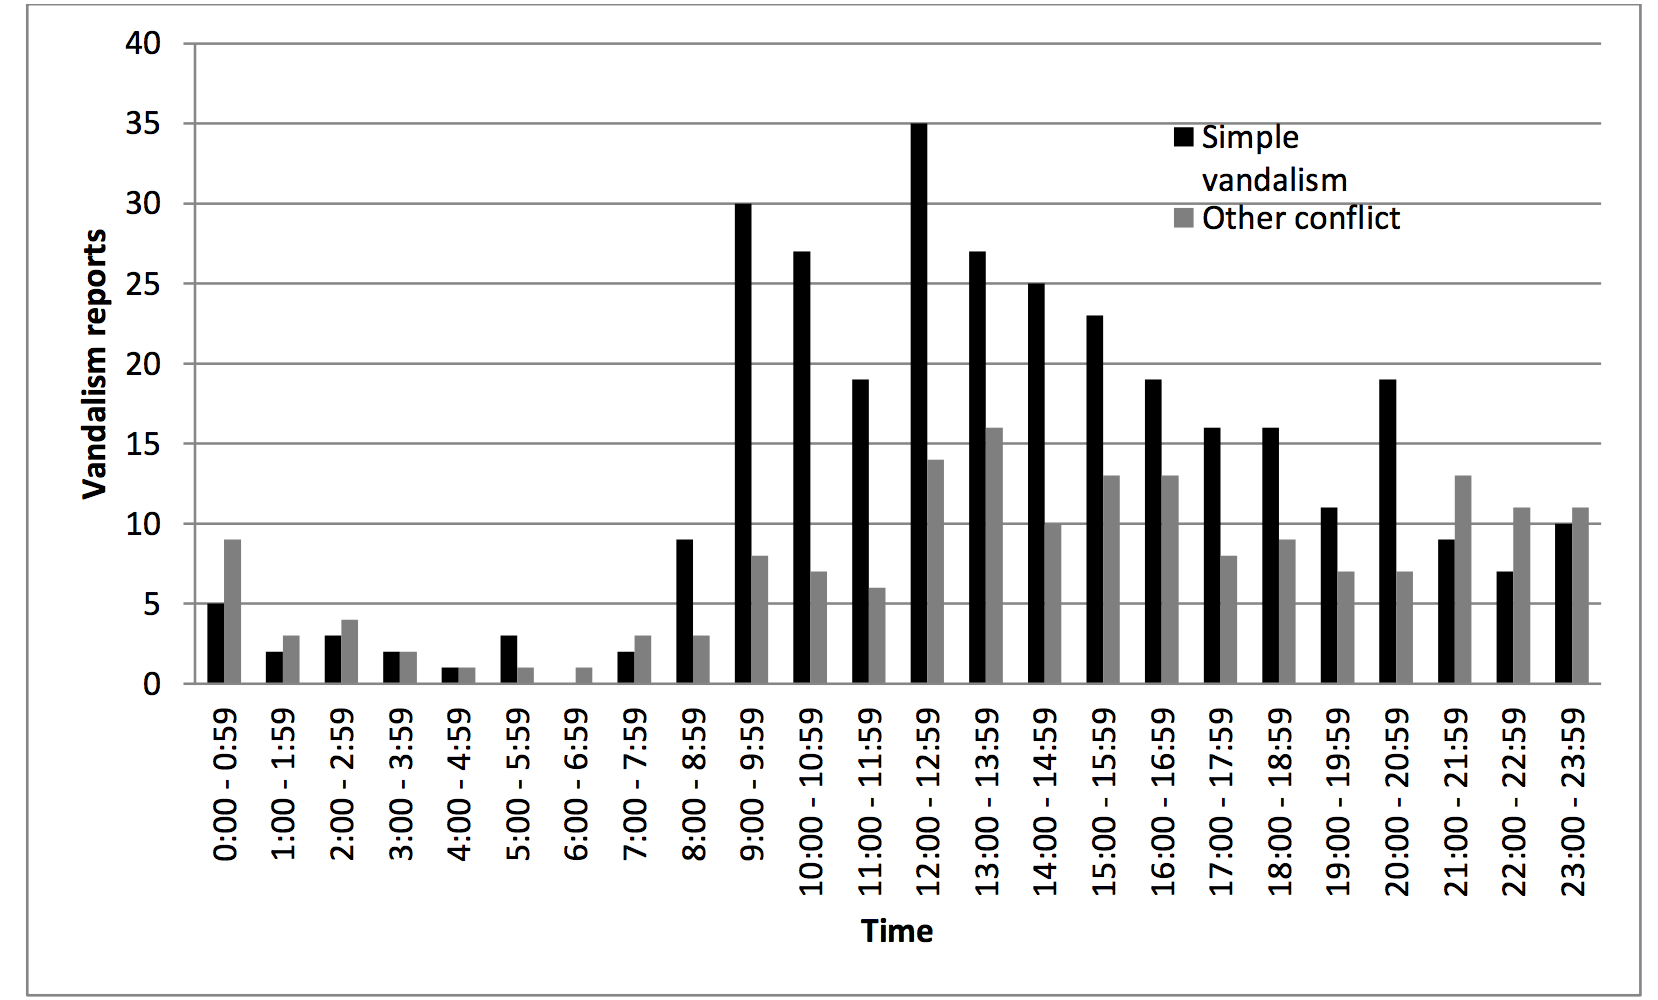
\includegraphics[scale=0.5]{simple.png}
\caption{Chart of simple vandalism over other conflict types\cite{main}}
\label{simple}
\end{figure}
The Fig.\ref{simple} gives an idea of simple vandalism and other conflicts over a weekday. We can see that simple vandalism is more during noontime i.e between 12 to 1. This is the time when schools and colleges have their break time. It is known from analysis of the IP-Ranges used by vandals that a lot of simple vandalism is performed from school computers. We can say lot of simple vandalism is from school computers but not completely because  also we can observe that it is also high during evenings.
\subsection*{Personal Attacks:}
In this type of conflict, instead of commenting on content of an article, editors comment on editor who wrote the content. Personal attacks are not allowed within the wikipedia community.  However, fierce disputes regularly escalate to intense argument and sometimes members of the community lose their temper. It is unpleasant to be personally attacked or treated uncivilly, but sometimes it happens because another user is angry. Personal attacks often cause the person being attacked to feel angry and often tempts to respond to a user who personally attacks you by defending yourself by attacking them back or reporting the user to a community noticeboard or by leaving an official 'warning' on the attacker's talk page. All of these things are usually unnecessary and serve only to escalate the conflict you're experiencing. Personal attacks are usually handled by administrators by temporal or in severe cases definite blocking of the offender's accounts.
\subsection*{General Conflict :}
General Conflict occurs when users call for Administrator action to get rid of opponents. In most cases, opposed are called as edit warriors or their contribution in discussion is taken as personal attack. Such conflicts often attract supporters of either side and can lead to fierce arguments, causing follow-up allegations of vandalism or personal attacks.
\section{Resolution for Conflicts}
Administrators play major role in resolution of these user conflicts and for preserving quality and content of an article. “Administrator Intervention against vandalism is a central page” where vandals and conflicts which are getting out of control are evaluated by administrators upon user’s request.  But the prerequisite to report on this page is, user should have given enough warnings to vandalizer before asking administrators involvement. Then the administrators will resolve these vandalism reports mainly by exploiting following methods\cite{main} depending on the severity of the conflict among the editors.
\begin{itemize}
\item[$\bullet$ ]Temporal blocking of IP address
\item[$\bullet$ ]Temporal blocking of user accounts
\item[$\bullet$ ]Infinite blocking of user accounts
\item[$\bullet$ ]Semi- blocking of articles
\item[$\bullet$ ]Complete blocking of articles
\item[$\bullet$ ]EOD (End of Discussion)
\item[$\bullet$ ]Reprimand (warning)
\item[$\bullet$ ]Archiving without action 
\end{itemize}
This Fig.\ref{resolutions} describes resolution methods over 500 reports. And by looking at it, estimation can be made that most frequent resolution method is Temporary IP block of vandalizer. Usually, Administrator don't want to anger users by choosing option of Indefinite(Permanent) User block and instead opts for Archived without action option, which is second most frequent resolution method. \\
\begin{figure}[h]
\centering
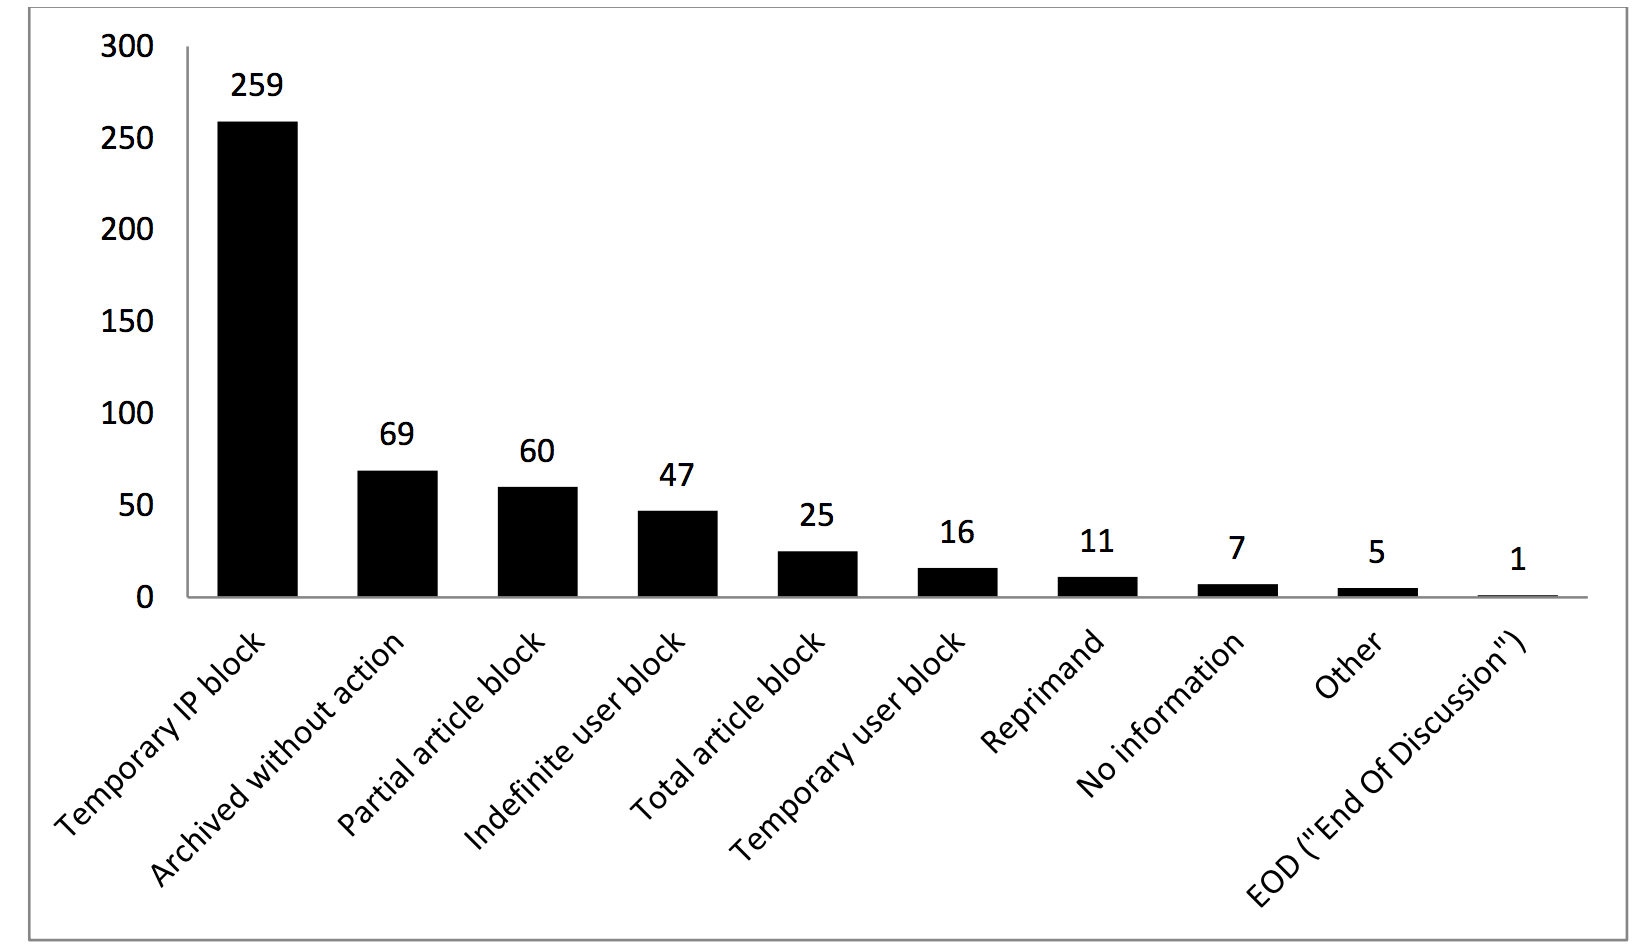
\includegraphics[scale=0.4]{resolutions.png}
\caption{Resolution methods\cite{main}}
\label{resolutions}
\end{figure} 
There are also another policies to get rid of conflicts, like 'Dispute Resolution' in which Administrator action is not involved.
\subsection*{Dispute Resolution:}This method describes following ways of solving disputes among editors\cite{dispute}. It tells:
\begin{itemize}
\item[$\bullet$ ]Approach the editors and explain why their edits are not appropriate in some cases.
\item[$\bullet$ ]Stay polite when talking with another editor and make use of article talk page or user talk page to talk with an editor.
\item[$\bullet$ ]It is useful to explain the reason along with edit summary to help understand reason behind edit you made. 
\item[$\bullet$ ]If you are reverting, explain yourself rather than starting an edit war.
\end{itemize}
\section*{Experiments}
In most of the case, unregistered user vandalise articles more frequently than registered user, $16\%$ to $1\%$ respectively. Researchers performed different experiments to prove it. By the research of authors of \cite{wiki}, authors observed that registered users contributed $67\%$ of these edits, while anonymous users contributed $33\%$. It can be explained by the following Fig.\ref{regular} of venn diagrams of Regular edits and Vandalism made with different vandalism actions of change, delete, insert on text of an article. Vandals are more likely in inserting text and are much less likely to make multiple changes in one revision.
\begin{figure}[h]
\centering
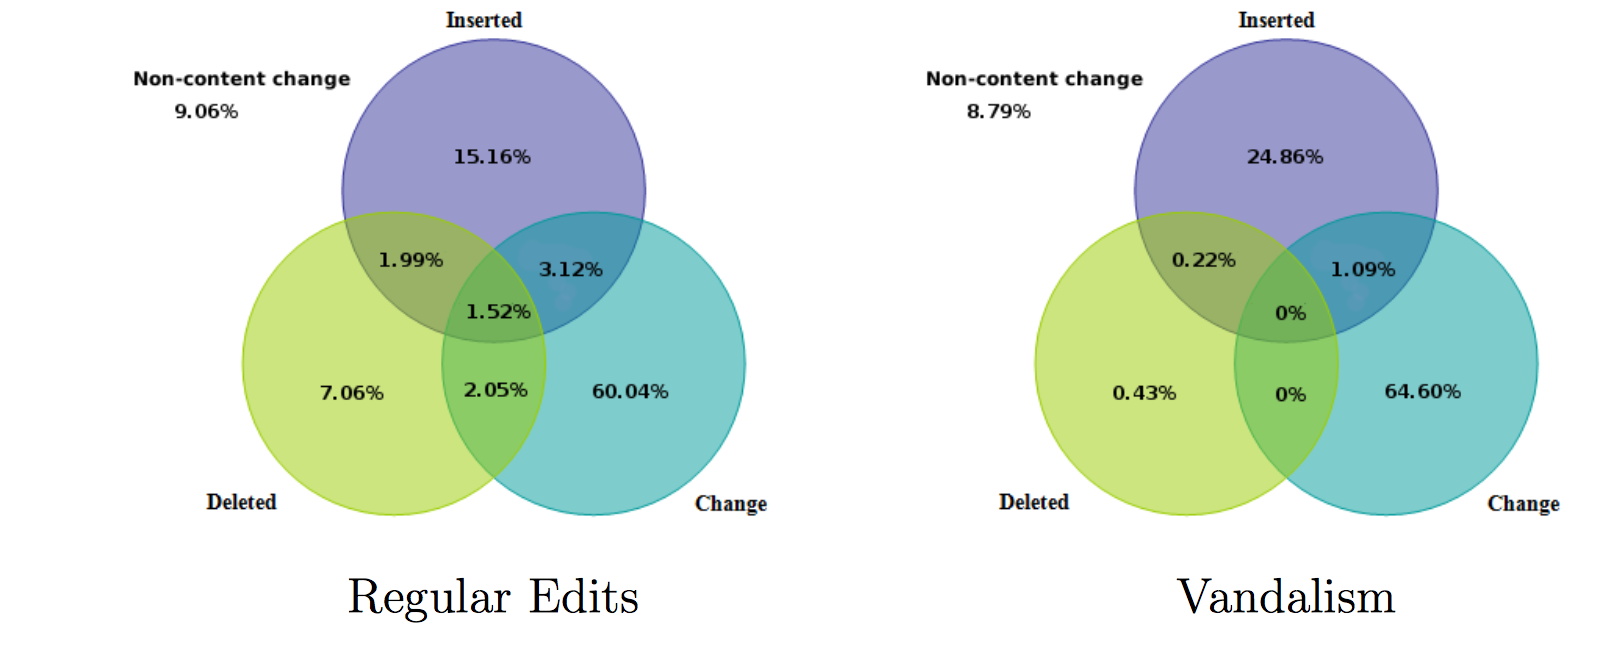
\includegraphics[scale=0.5]{regular.png}
\caption{Regular and vandalized edits\cite{wiki}}
\label{regular}
\end{figure}
One of the feature  according to top $10$ features of information gain is change in sentiment.
\begin{figure}[h]
\centering
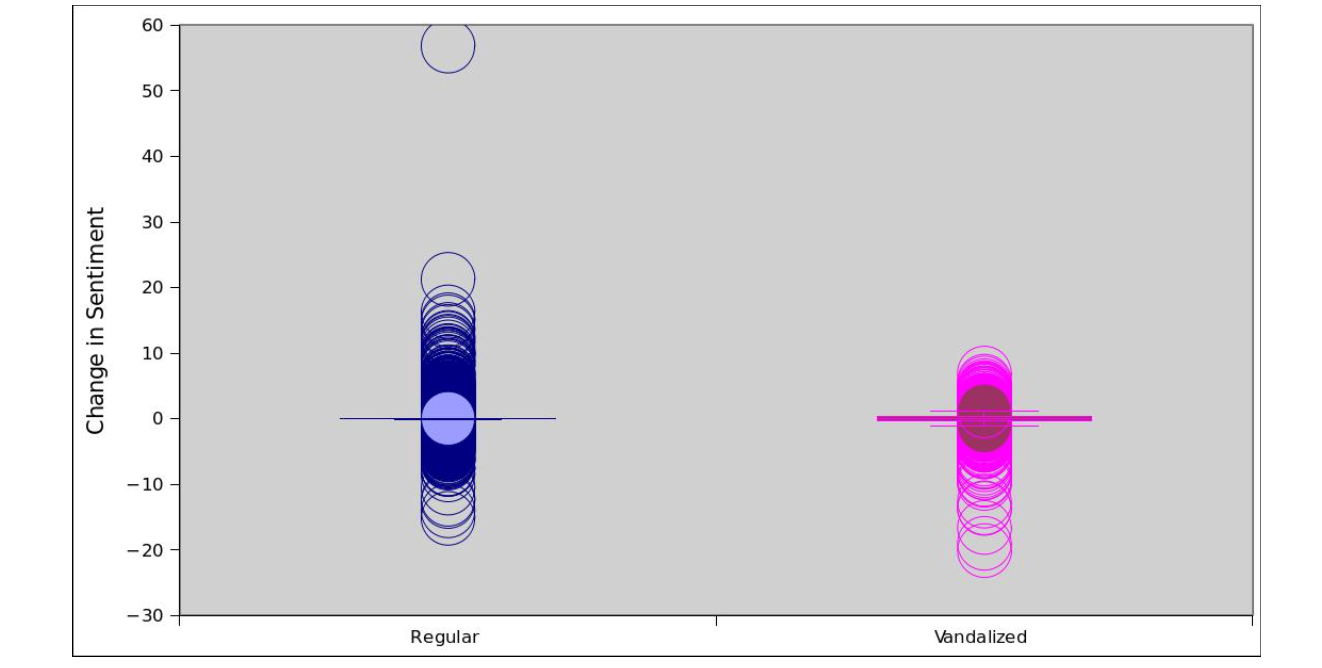
\includegraphics[scale=0.5]{sentiment.png}
\caption{change in sentiment\cite{wiki}}
\label{sentiment}
\end{figure}
The Fig.\ref{sentiment} shows the values of the change in sentiment score. Authors of \cite{wiki}note that for vandalising edits, the mean change in sentiment was $−0.14$ with a standard deviation of $2.0$ and for regular edits the mean change was $0.03$ with a standard deviation of $1.1$. Most edits of vandalism or regular edits had zero change in sentiment score. By observing at Fig.\ref{sentiment} we can also tell that vandalism moves more towards a negative change in sentiment while regular edits moves towards a positive change.\\
Then the another experiment of authors of \cite{active} who used two classifiers: Logistic regression and SVM  by taking two revision histories : “Microsoft” and “Abraham Lincoln”. Fig.\ref{classifier},the table shows the distribution of types of vandalism for this classification methods.
\begin{figure}[h]
\centering
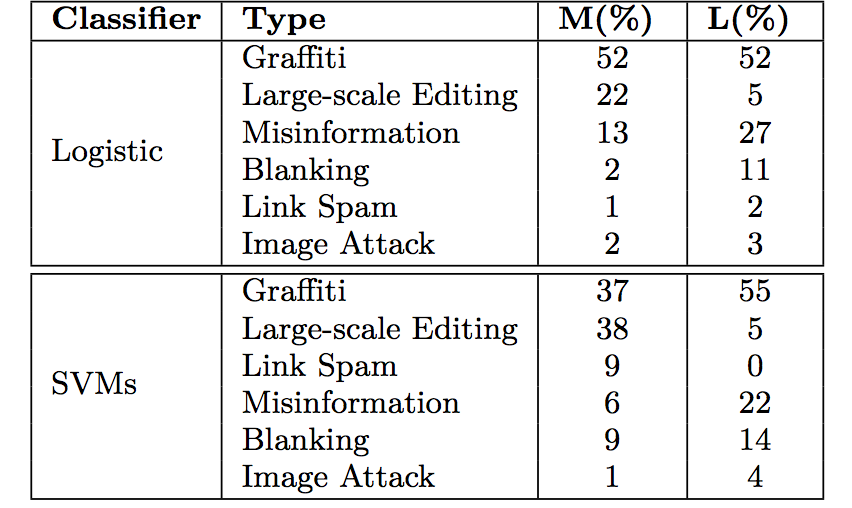
\includegraphics[scale=0.5]{classifier.png}
\caption{classification methods\cite{active}}
\label{classifier}
\end{figure}
Both methods are strong in detecting large scale and small scale vandalism instances. And the classifiers are also successful in identifying various misinformation vandalism occurrences like removing an alphabet from a name( Ex: Removing T from Robert and making it Rober), replacing existing name entities with irrelevant names(Ex: replacing Mary with dory), changing date information(Ex: change birthday from April 1 to may 1) etc. By looking at the result, we can tell that the possibility of tuning a classifier with language model statistics features to classify these types of vandalism is possible.
\section{Conclusion}
This paper gives the clear understanding of vandalism and about the factors which cause vandalism in Wikipedia articles. Following various user access levels and their duties towards protection of content of an article. Also about various methods to detect and get rid of Vandalism. Later it explains about various types of conflicts among wikipedia users and administrator action to resolve those conflicts following experiments made by researchers.\\  
Wikipedia founder Jimmy Wales has stated in an interview, the vision of Wikipedia is 'a world in which every single person on the planet is given free access to the sum of all human knowledge. That’s what we’re doing.'  As anyone can edit Wikipedia, most of the time that's a good thing because millions of people have made positive contributions but then there is problem with some people who add incorrect information, deliberately or by mistake.  Administrators play major role in resolving conflicts among the Wikipedia users and there are vandalism detectors to detect vandalism and recover it quickly. This way quality of content is preserved. 

%\input{samplebody-conf}
\begin{thebibliography}{9}

\bibitem{O'Sullivan}
Dan O'Sullivan, (2009). 
\textit{Wikipedia: A new community of practice?}, International Sociology 2005.

\bibitem{alexa}
\url{https://en.wikipedia.org/wiki/List_of_most_popular_websites}.
[Online; accessed 15-Jan-2018]
\bibitem{german}
\url{https://en.wikipedia.org/wiki/German_Wikipedia}.[Online; accessed 6-Nov-2017]
 
 \bibitem{Harpalani}
 Manoj Harpalani, Michael Hart, Sandesh Singh, Rob Johnson and Yejin Choi (2011)
\textit{Language of Vandalism: ImprovingWikipedia Vandalism Detection via Stylometric Analysis}.Proceedings of the 49th annual meeting of the Association for Computational Linguistics: Human language technologies (pp. 83–88). Portland, OR.
 
\bibitem{help}
\url{http://www.wikiwand.com/en/Help:Wikipedia:_The_Missing_Manual/Editing,_creating,_and_maintaining_articles/Who_did_what:_Page_histories_and_reverting}
[Online; accessed 8-Nov-2017]

\bibitem{anthology}
\url{https://aclweb.org/anthology/P/P11/P11-4017.pdf}[Online; accessed 13-Nov-2017]

\bibitem{active}
Si-Chi Chin,W. Nick Street,Padmini Srinivasan,David Eichmann.
\textit{Detecting Wikipedia Vandalism with Active Learning and Statistical Language Models}.In: WICOW ’10: Proc. of the 4th Workshop on Information Credibility on the Web. (Apr 2010).

 
 \bibitem{vandalism} 
 \url{https://en.wikipedia.org/wiki/Wikipedia:Vandalism}[Online; accessed 28-Nov-2017]
  \bibitem{vandalsim2} 
 \url{https://rstudio-pubs-static.s3.amazonaws.com/72433_8b472f77a2b74ac3a975e3a0e3f49374.html}[Online; accessed 8-Dec-2017]
\bibitem{user}
\url{https://en.wikipedia.org/wiki/Wikipedia:User_access_levels}
[Online; accessed 28-Nov-2017]
\bibitem{main}
T.Roessing.
\textit{Vandalism and conflict resolution in Wikipedia. An empirical analysis on how a large-scale web-based community deals with breaches of the online peace}
.IADIS International Conference “Web Based Communities and Social Media 2011” in Rome, Italy July 22-24, 2011.
\bibitem{creating}
R. Priedhorsky, J. Chen, S. T. K. Lam, K. Panciera, L. Terveen, and J. Riedl.
\textit{Creating, destroying, and restoring value in Wikipedia.}In Proceedings of the International ACM Conference on Supporting Group Work, pages 259–268, Sanibel Island, Florida, USA, 2007. ACM.
\bibitem{potthast}
Martin Potthast, Benno Stein, and Teresa Holfeld. 2010.
\textit{Overview of the 1st International Competition on Wikipedia Vandalism Detection.}
\bibitem{char}
Nathaniel Miller.
\textit{Characterizing Conflict in Wikipedia(2012)}.
\bibitem{engagement}
Joachim Schroer ,Guido Hertel 2007.
\textit{Voluntary Engagement in an Open Web-based Encyclopedia: Wikipedians, and Why They Do It}.
\bibitem{dispute}
\url{https://en.wikipedia.org/wiki/Wikipedia:Dispute resolution}.[Online; accessed 12-Dec-2017]
\bibitem{wiki}
Manoj Harpalani, Thanadit Phumprao, Megha Bassi, Michael Hart, and Rob Johnson.\textit{Wiki Vandalysis - Wikipedia Vandalism Analysis Lab Report for PAN at CLEF 2010}
\bibitem{revert}
E.Borra et. el., \textit{Contropedia - the analysis and visualization of controversies in Wikipedia articles, OpenSym 2014 Proceedings}


\end{thebibliography}











\end{document}




















